
\section{Related Work}
\label{sec:relatedwork}
\textbf{Efficient Neural Network.}
There are several different approaches 
to reduce the memory footprint, latency, and power of modern NN 
architectures.
These techniques can be broadly categorized into:
(1) pruning~\cite{han2015learning, li2016pruning, mao2017exploring, lecun1990optimal, molchanov2016pruning, yang2017designing,michel2019sixteen, fan2019reducing, gordon2020compressing, raganato2020fixed, mao2020ladabert, sanh2020movement};
(2) knowledge distillation~\cite{hinton2015distilling, mishra2017apprentice, polino2018model, romero2014fitnets,sanh2019distilbert, sun2019patient, jiao2019tinybert, tang2019distilling, turc2019well, sun2020mobilebert, wang2020minilm, xu2020bert};
(3) efficient neural architecture design~\cite{iandola2016squeezenet, sandler2018mobilenetv2, tan2019efficientnet, howard2019searching, lan2019albert, dehghani2018universal};
(4) hardware-aware NN co-design~\cite{han2017efficient,gholami2018squeezenext, kwon2018co}; and
(5) quantization.

Here, we only focus on quantization and briefly discuss the related work.


%%%%%%%%%%%%%%%%%%%%%%%%%%%%%%%%%%%%%%%%%%%%%%%%%%%%%%%%%%%%%%%%%%%%
\begin{figure*}
\centering{
  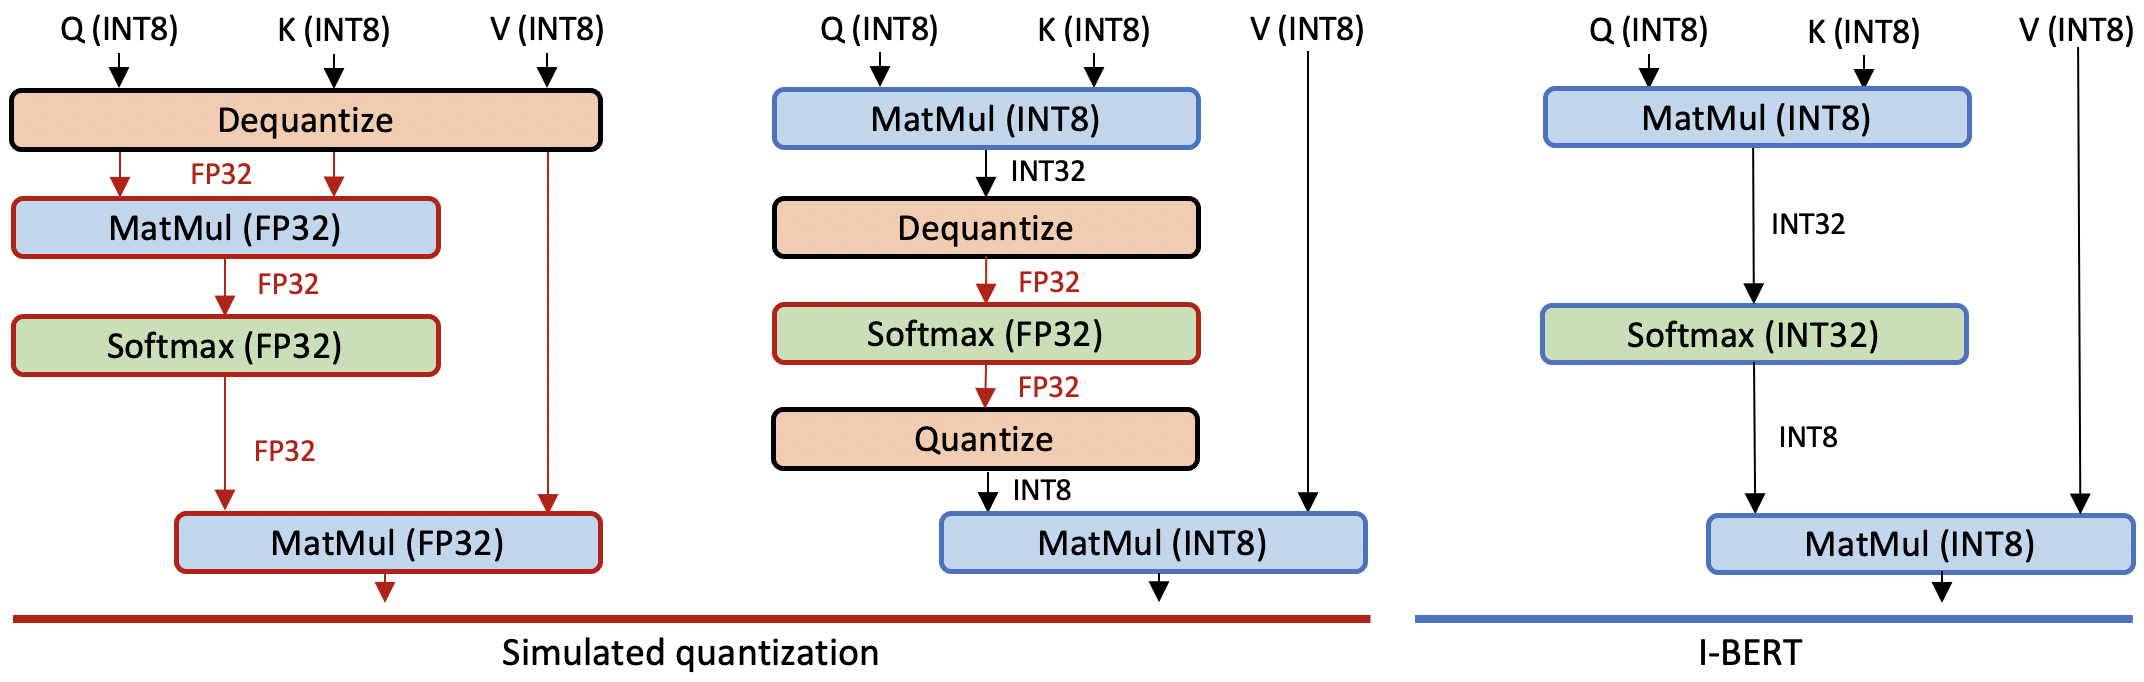
\includegraphics[width=0.95\textwidth]{figures/overview.png}
  \vskip -0.15in
  \caption{Comparison of different quantization schemes applied to the self-attention layer in the Transformer architecture. 
  (Left) Simulated quantization, where all operations are performed with floating point arithmetic. 
  Parameters are quantized and stored as integer, but they are dequantized into floating point for inference. 
  (Middle) Simulated quantization, where only a part of operations are performed with integer arithmetic. 
  Because the Softmax in this figure is performed with floating point arithmetic, the input to the Softmax should be dequantized; and the output from the Softmax should be quantized back into integer to perform the subsequent integer MatMul.
  (Right) The integer-only quantization that we propose. 
  There is neither floating point arithmetic nor dequantization during the entire inference.
  }
  \label{fig:overview}
  }
  \vspace{-3mm}
\end{figure*}
%%%%%%%%%%%%%%%%%%%%%%%%%%%%%%%%%%%%%%%%%%%%%%%%%%%%%%%%%%%%%%%%%%%%


\textbf{Quantization.}
For quantization, the parameters and/or activations are represented with low bit precision~\cite{choi2018pact, courbariaux2015binaryconnect, dong2019hawq, jacob2018quantization, rastegari2016xnor, zhang2018lq, zhou2016dorefa, li2016ternary, wu2016quantized, courbariaux2016binarized, wang2018haq}.
While this line of research mostly focuses on CNN models, there have been recent attempts to introduce quantization techniques into Transformer based models as well.
For example, \cite{bhandare2019efficient} and~\cite{zafrir2019q8bert} propose an 8-bit quantization scheme for Transformer based models and compress the model size up to 25\% of the original size.
Another work~\cite{shen2020q} applies uniform and mixed-precision to quantize BERT model,
where a second-order sensitivity method is used for the mixed-precision setting.
\cite{fan2020training} quantizes a different subset of weights in each training iteration to make models more robust to quantization.
Recently, there have been attempts to quantize BERT with even lower precision. 
\cite{zadeh2020gobo} presents a 3/4-bit centroid-based quantization method that does not require fine-tuning.
\cite{zhang2020ternarybert,bai2020binarybert} leverage knowledge distillation~\cite{hinton2015distilling} to ternarize/binarize weights. 
\cite{jin2021kdlsq} combines knowledge distillation and learned step size quantization~\cite{esser2019learned} method to achieve up to 2-bit quantization of BERT. 



However, to the best of our knowledge, all of the prior quantization work on Transformer based models use \textit{simulated quantization} (aka fake quantization), where all or part of operations are performed with floating point arithmetic.
This requires the quantized parameters and/or activations to be dequantized back to FP32 for the floating point operations. 
For example, \cite{shen2020q, zadeh2020gobo} perform the entire inference using floating point arithmetic, as schematically shown in~\fref{fig:overview} (left).
While~\cite{bhandare2019efficient, zafrir2019q8bert, zhang2020ternarybert, bai2020binarybert} attempt to process Embedding and MatMul efficiently with integer arithmetic, they keep the remaining operations (i.e., GELU, Softmax, and LayerNorm) in FP32, as illustrated in~\fref{fig:overview} (middle).
However, our method \OURS uses integer-only quantization for the entire inference process---i.e., without any floating point arithmetic and without any dequantization during the entire inference.
This is illustrated in~\fref{fig:overview} (right). 
This allows more efficient hardware deployment on specialized accelerators or integer-only processors~\cite{armcortexm} as well as faster and less energy consuming inference. 
While we focus on uniform quantization, our method is complementary to other mixed and/or low-precision methods, and can be deployed for those settings as well.


To briefly discuss, there are also several quantization works for computer vision.
\cite{jacob2018quantization} introduces an integer-only quantization scheme for popular CNN models,
by replacing all floating point operations (e.g., convolution, MatMul, and ReLU) with integer operations.
Similarly, the recent work of~\cite{yao2020hawqv3} extends this approach to low precision and mixed precision dyadic quantization, which is an extension of integer-only quantization where no integer division is used.
However, both of these works are limited to CNN models that only contain linear and piece-wise linear operators, and they cannot be applied to Transformer based models with non-linear operators, e.g., GELU, Softmax, and LayerNorm. 
Our work aims to address this limitation by extending the integer-only scheme to the Transformer based models without accuracy~drop.